%-*- coding: UTF-8 -*-
% !TEX program  = xelatex

\documentclass{thesis-cqjtu}

\title{重庆交通大学本科学位论文 \XeLaTeX 模板}    % 标题
\college{航运与船舶工程学院}                    % 学院
\major{船舶与海洋工程}                          % 专业
\articleclass{论文}                           % 分类:论文/设计
\author{可莉}                                 % 作者姓名
\authorno{631800000000}                       % 学号
\date{2028年5月27日}                           % 完成日期
\instructor{琴}                              % 指导教师
\reviewer{凯亚}                                  % 评阅教师

\usepackage{lipsum}     % 生成随机文本,可删除
\usepackage[none]{hyphenat} % 英文单词不从中间断开, 配合 \sloppy 使用
\begin{document}
\sloppy % 让字符间距不严格一致,保证两端对齐

% 封面、原创声明和授权、摘要、目录
\makecover
\pagenumbering{Roman}
\originality

\begin{cnabstract}
    随着经济与科技的快速发展,本文基于哈哈哈,主要工作如下:
    \begin{enumerate}
        \item 归纳总结啊啊啊;
        \item 建立变变变模型,详细阐述了吃吃吃;
        \item 根据哒哒哒,进行计算分析;
    \end{enumerate}

    通过啊啊啊结果,得到了如下结论:

    \begin{enumerate}
        \item 叭叭叭呈正相关;
        \item 哒哒哒;
        \item 呃呃呃最大可降低了76\%的疼疼疼;
    \end{enumerate}

    \cnkeywords{LaTeX;学位论文;论文排版;有限元仿真}
\end{cnabstract}

\begin{enabstract}
[The Subject of Undergraduate Graduation Project (Thesis) of CQJTU]% 这里填英文标题
% 这里是英文摘要正文
\lipsum % 生成随机文本


     \enkeywords{LS-DYNA; Ship collision; Finite element simulation}
\end{enabstract}

% 目录
\tableofcontents

% 正文
\clearpage
\pagestyle{plain}
\afterpage{\pagestyle{plain}} % 防止多页目录时后面格式不正确
\pagenumbering{arabic}

\section{绪\qquad{}论}

\subsection{研究背景及意义}
研究背景及意义。
参考文献引用\upcite{刘海洋latex入门}。
\subsection{研究现状}
研究现状。
\subsection{本章小结}
本章小结。

\section{有限元模型的建立}

\subsection{集装箱船有限元模型的建立}
本文选取12300t内河集装箱船作为研究对象,该船的主要参数如表~\ref{tab:ShipParams}~所示。该集装箱船的空船重量为9000t,载重量为3300t。
\begin{table}[htb]
    \centering
    \small \linespread{1.2} \selectfont % 调整字体大小、行间距
    \caption{集装箱船的主要参数}
    \begin{tabular}{@{}cc@{}}
    \toprule
        \makebox[0.3\textwidth]{参数名称}	    &    \makebox[0.3\textwidth]{数值}     \\ \midrule
        总长 $L_{OA}$	    &    163.9 m     \\
        垂线间长 $L_{PP}$	&    159.5 m     \\
        型宽 B	        &    26.1 m     \\
        型深 D	        &    15.6 m     \\
        吃水 T	        &    5.6 m     \\
        排水量 $\Delta$	    &    12300 t     \\
        肋距 FS	        &    780 mm     \\ \bottomrule
\end{tabular}
\label{tab:ShipParams}
\end{table}

\subsubsection{图片测试}
这里写一段文字,文字文字文字文字文字文字文字文字文字文字文字文字。如图~\ref{fig:energy_a}~所示,请\textbf{不要}在正文中书写“如\textbf{下}图/表所示”,因为图片或表格会飘到合适的位置以保证排版美观。

\begin{figure}[htb]
    \centering
    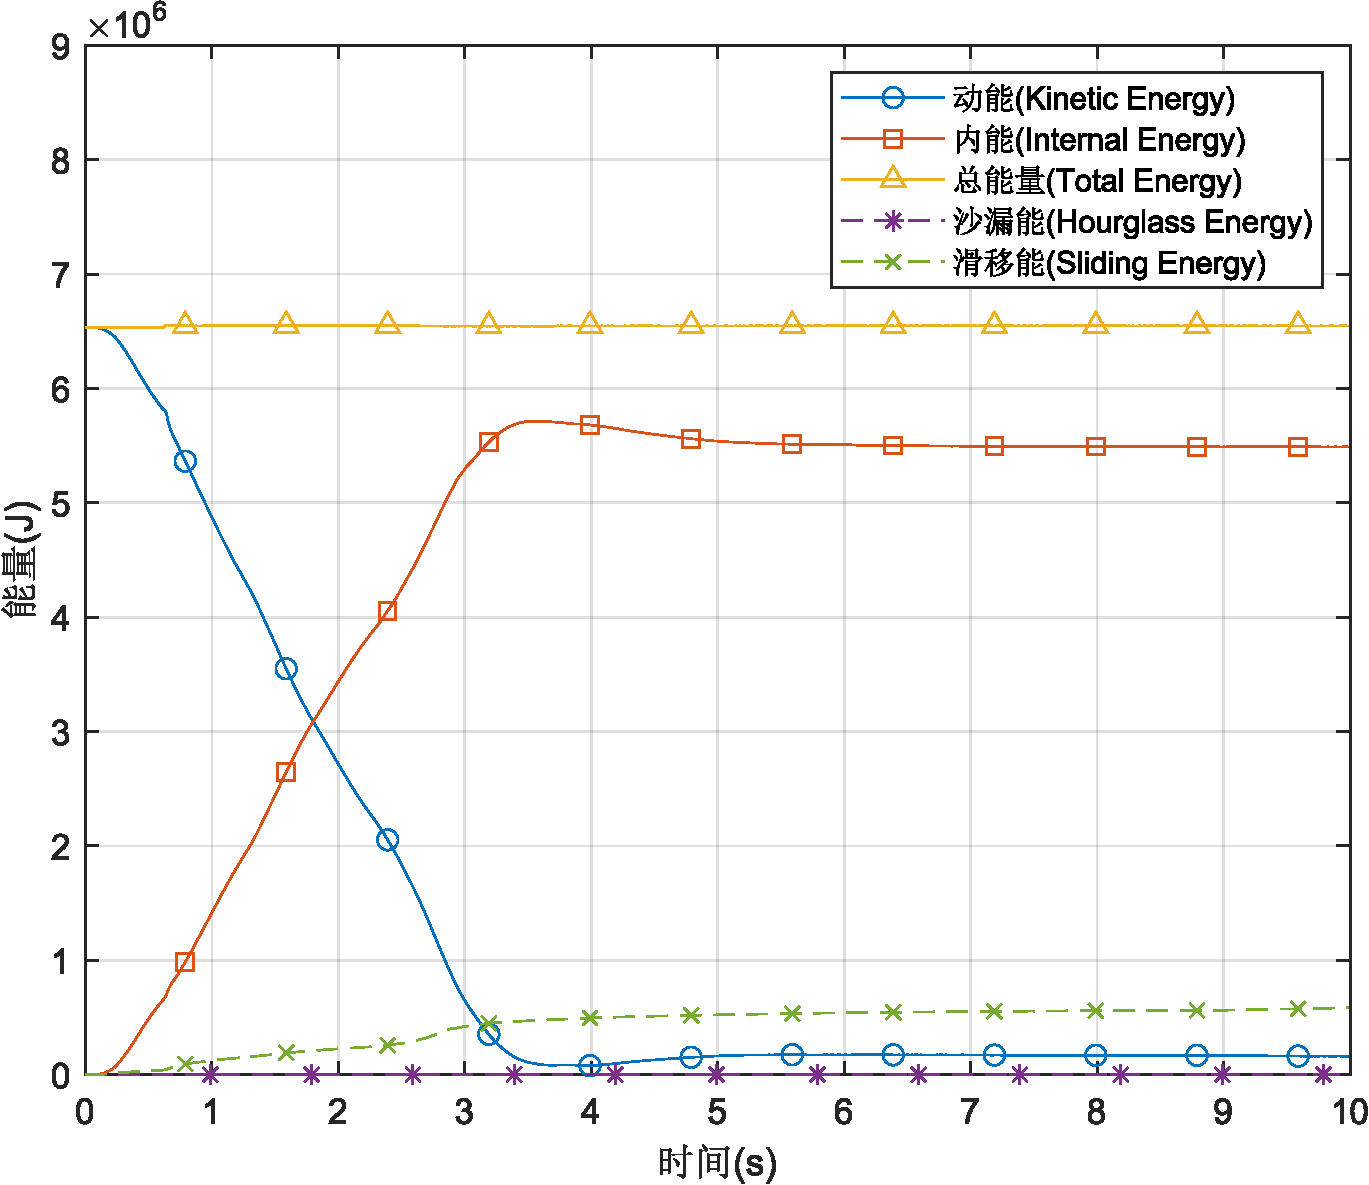
\includegraphics[width=0.8\textwidth]{figures/energy-crop.pdf}
    \caption{这里是图片的描述}
    \label{fig:energy_a}
\end{figure}

在时间 $t=0$ 时刻,有初始状态:
\begin{align}
    x_i(X_\alpha,0) &=X_\alpha              \\
    \dot{x}_i (X_\alpha,0) &= V_i (X_\alpha)
\end{align}

其中 $V_i (X_\alpha)$ 为该点的初始速度。

$\delta_{ij}$ 是克罗内克符号,其定义如下:
\begin{equation}
    \delta_{ij} = 
    \left\{
        \begin{array}{l}
            1 \qquad i = j   \\
            0 \qquad i \neq j 
        \end{array}
    \right.
\end{equation}

如果向蒙德的酒客们说起西风骑士团战力最强的成员,恐怕大多数人会列举大名鼎鼎的代理团长琴、骑兵队长凯亚或神秘的贵公子迪卢克。

但也有人在醉眼朦胧间,目睹了一位红色骑士将整座望风山夷为平地的壮举——

若想寻访这位神秘的骑士,恐怕就要到西风骑士团的禁闭室一探究竟了。假如禁闭室空空如也,或许某些爆炸性的糟糕事件就快要发生了…

可莉就是这样的「危险人物」。作为骑士团正式成员,她的能力不容小觑。而作为一个过于活泼的孩子,她的破坏力同样巨大。毕竟,与蒙德其他小孩子不同,爆炸物才是可莉最为喜欢的玩具。


\nsection{结\qquad{}论} % 设计类为“设计总结”
论文类为“结\qquad{}论”,设计类为“设计总结”,\textbf{没有}章节序号!这是个很有特色的设计。

% 致谢要加入到目录,但是无章节号,nsection 为模板定义的环境,自动加入目录
\nsection{致\qquad{}谢}
听我说,谢谢你……

% 参考文献
{
    \linespread{1.2} \selectfont    % 缩小行间距以美观,如需严格按照模板要求,请注释掉此行
    \zihao{5}
    \bibliographystyle{gbt7714-numerical}
    \bibliography{example}
    \addcontentsline{toc}{section}{参~考~文~献}    % 加入到目录
}

% 附录
\appendix
\section{所有数据}

啦啦啦啦啦。如果没有附录记得删掉!

\section{程序代码}

啦啦啦啦啦。如果没有附录记得删掉!

\end{document}